\documentclass[titlepage,a4paper,12pt]{book}

\usepackage[utf8]{inputenc}
\usepackage[catalan]{babel}
\usepackage{graphicx}
\usepackage{marvosym}
\usepackage{listings}
\usepackage{textcomp}
\usepackage[]{color}
\begin{document}
\tableofcontents
\chapter{Algorismes Evolutius\label{GA}}

En aquest capítol es farà una repàs de que es coneix com algorismes evolutius
\cite{H75}. S'explicarà una de les dos filosofies existents,
algorismes genètics Darwinistes (GA) i es farà una introducció a Genetic
Expression programming (GEP), on per explicar aquest segon tipus d'algorismes
s'introduiran els algorismes de programació genètica (GP), que és l'origen del
que va partir GEP.

\section{Introducció}
Els algorismes genètics són eines evolutives, que es poden
classificar dins del camps de la intel·ligència artificial i que es solen usar
en problemes d'optimització. La filosofia d'aquesta família d'algorismes és
basar-se en els mecanismes de selecció natural que Darwin ja va presentar en el
llibre \emph{The Origin of Species}, És a dir, els individus que millor
s'adapten a l'entorn són aquells que sobreviuen amb major facilitat.
Conseqüentment també produeixen més descendència, la qual cosa provoca que, de
mica en mica, els trets diferencials que caracteritzen als bons individus es van
propagant per la població i a través dels seus descendents.

En els algorismes evolutius, les solucions al problema són codificades com a
individus d'una població, tal i com es veurà més endavant. Posteriorment,
simulant les diferents fases per la que passa la reproducció natural, i aplicant
tècniques que provoquen un cert grau de pressió selectiva (supervivència dels
més forts), aquestes van evolucionant cap a solucions al problema més bones.
Els primers fonaments dels GA van ser proposats per Holland \cite{H75} al 1975.
Aquests algorismes aconsegueixen evolucionar els individus de tal manera que el
grau d'adaptació a l'entorn (avaluació o \emph{fitness}) va augmentant de
generació en generació.

\section{Algorismes genètics Darwinistes}

Els algorismes genètics Darwinistes segueixen l'esquema de funcionament clàssic
dels algorismes genètics. En aquests, s'intenta imitar els processos de la
evolució natural sense cap altra modificació conceptual. Normalment, quan es
parla del terme algorisme genètic es refereix a aquest primer model de
funcionament. En l'actualitat els GA han estat molt utilitzats en gairebé tots
els àmbits de la ciència com a eina per optimitzar o buscar bones solucions
comparables a les actualment disponibles. En l'àmbit de la bioinformàtica és una
de les àrees d'aplicacions reals on més s'han utilitzat
\cite{PSBE01,D96,wgl:2000,WWBG95}.

\subsection{Principis bàsics}

Els GA es recolzen en tres pilars bàsics: el primer d'ells és la selecció
d'individus de la població, el segon el creuament d'individus i el tercer la
funció d'avaluació. La selecció és important perquè és el mètode per escollir
els individus que generaran descendència, seria bo que normalment aquests
individus fóssin els millors adaptats a l'entorn. És a dir, aquells amb un
\emph{fitness} més alt.  Això, junt amb el creuament de les solucions
seleccionades, progressivament fa evolucionar la població de solucions. La
funció d'avaluació és el mecanisme amb el qual es computa el grau d'adaptació de
cada individu a l'entorn.

Del paràgraf anterior es pot deduir que els GA són algorismes no deterministes.
Això és el resultat dels mecanismes estocàstics emprats. I això pot comportar
que no sempre s'assegura l'obtenició del màxim global de la funció que es vol
optimitzar, la qual cosa és certa, però el que sí que s'ha demostrat
empíricament és que normalment sempre s'arriben a solucions bones amb un temps
molt menor que hagués trigat un algorisme de cerca sistemàtic \cite{BBM93}. 

\subsubsection{Representació dels individus}

Continuant amb les analogies biològiques, la representació de les solucions es
fa emprant cromosomes. Aquests estan formats per la concatenació de gens. Cada
gen representa el valor d'un paràmetre (o variable de decisió) d'una possible
solució.  Per exemple, si estem definint les proporcions òptimes per a una
caixa, un cromosoma podria venir definit per les següents variables:
(altura,amplada,profunditat). Cada solució hauria d'estar perfectament definida
en el seu cromosoma.

Al cromosoma també se'l coneix com genotip, ja que representa un conjunt de
qualitats o atributs de la solució que no s'expressen en la realitat (en aquest
cas la realitat s'entén com la simulació necessària per avaluar un cromosoma).


%Podria ser que l'hora de simular el cromosoma, s'adoptaren una serie de
%qualitats no definides al cromosoma de forma aleatòria, o indeterministes.  Com
%per d'exemple, es pot imaginar un cromosoma o genotip on els seus gens són els
%aminoàcids que composaran una cadena peptídica. El fenotip serà l'estructura
%tridimensional que aquesta molècula adoptarà a l'espai, que no necessàriament ha
%d'estar codificada al cromosoma.

\subsubsection{Esquema bàsic}

Com s'ha comentat anteriorment, un GA imita el cicle de la evolució natural
proposat per Darwin. Aquest cicle bàsicament es pot resumir en cinc fases:
inicialització, avaluació, selecció, creuament i mutació. Cadascuna de les quals
es descomposa en altres subfases que seran explicades en la secció
\ref{subsec:operadors}. La figura \ref{fig:ga} es mostra el diagrama
d'activitats que segueix un GA.

\begin{figure} \centering 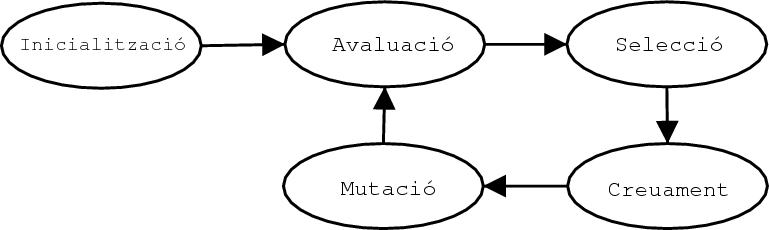
\includegraphics[width=4in]{intro/ga}
\caption{\label{fig:ga}Diagrama d'activitats d'un algorisme genètic}
\end{figure}

A grans trets, la fase d'inicialització, crea la població inicial que començarà
el procés evolutiu. Sempre cal un conjunt suficientment gran i divers per
assegurar l'èxit del procés evolutiu \cite{G02}.

Pel que fa a l'avaluació, cal dir que és un dels aspectes més importants d'un
GA, en l'apartat \ref{subsec:avaluacio} s'entrarà amb molt més detall amb aquest
afer, però cal comentar abans que la funció d'avaluació és en si mateix el
problema que es vol resoldre o optimitzar.

La selecció és el mecanisme que tria els individus que seran candidats a ser
escollits, més endavant s'entrarà en molt més detall en els mecanismes
involucrats en la selecció desenvolupada, i també es citaran altes tècniques de
selecció.

El creuament és el procés pel qual es combinen dos cromosomes que s'han
seleccionat per tenir descendència. Hi han moltes formes de fer-ho, però una de
les més habituals és un creuament discret amb un o dos punts de tall.  Aquesta
és la tècnica que hem usat en dos dels nostres projectes \texttt{Pholus} i
\texttt{Chiron}  %% refs

Finalment, ve la mutació, que és l'encarregada d'introduir o canvis aleatoris en
els individus amb una probabilitat més aviat baixa. Aquesta activitat és
realitza per estar segurs de que tot l'espai de cerca pugui ser explorat.
Modificant la probablilitat d'aparició de mutacions donem més o menys
variablilitat genètica al algorisme, afavorint o desfavorint la convergència de
la població.

En acabar la mutació el cicle es tanca, i va iterant fins que la condició
d'aturada s'assoleix. Normalment la condició d'aturada és generar un nombre
prefixat de generacions, però alguns cops també s'utilitzen criteris, com per
exemple la convergència de la població.

\subsubsection{La funció d'avaluació\label{subsec:avaluacio}} La funció
d'avaluació és vital per un algorisme genètic. Aquesta tracta de simular
l'entorn en el qual estan immerses les solucions, i ens retorna el
\emph{fitness} o el grau d'adaptació dels individus a l'entorn. Cal fer notar
que la funció d'avaluació codifica el problema que es vol que el GA resolgui.

En alguns problemes la funció d'avaluació és tan complexa que s'ha de
simplificar per aproximacions més ràpides. Fins i tot en alguns casos s'ha
observat que el fet de substituir la funció d'avaluació per una menys complexa
dóna la oportunitat d'avaluar més individus per unitat de temps, i amb aquest
increment dels individus avaluats, al final s'assoleix una solució real més
acurada que la que es va trobar utilitzant la funció d'avaluació inicial
\cite{G89}. 

\subsubsection{Reproducció} En la reproducció estan implicats dos dels tres
pilars fonamentals dels GA, la selecció i el creuament. La creació de nova
descendència és un factor crític, en la mesura que de generació en generació,
els nous individus creats van superant als seus ascendents.

A partir d'ara entra en joc el concepte de pressió selectiva. És a dir, la
pressió que d'alguna manera s'exerceix sobre la població per a que vagi
augmentant el seu grau d'adaptació a l'entorn. Sovint s'ha de vigilar amb la
pressió selectiva, per que si és massa elevada, l'algorisme no té altra
escapatòria més que arribar a solucions bones a curt termini però que no
assoleixen els màxims globals. Aquestes solucions queden estancades en màxims
locals. D'altra banda si la pressió selectiva és molt baixa, el temps de
convergència és molt llarg.  Com sempre, s'ha d'arribar a un nivell de
compromís, entre el temps de convergència i el risc de caure en màxims locals.

Cal fer notar que de vegades podria ser que alguns individus siguin seleccionats
repetits cops en una mateixa generació. Això no té per que ser dolent, ja que
normalment aquests tipus d'individus tindran un \emph{fitness} molt alt.

Quan els individus que van a ser creuats ja han estat seleccionats, sols queda
pendent emparellar en grups de dos els individus per tal de generar nova
descendència. 

Un concepte que també s'ha d'introduir és el concepte d'\texttt{elitisme}, que
implica guardar els $k$ millors individus de la població de generació en
generació, així s'assegura que els millors individus de la població no es perden
mai.  Aquest és un element que afegeix presió evolutiva, mantenint un ``llistó''
del que no es baixa mai generació a generació, i accelerant la convergència.

\subsubsection{Convergència} 

Normalment els individus d'un GA van convergint cap als màxims de la solució de
generació en generació. Es diu que un GA ha convergit quan el 95\% de la
població té el mateix valor \cite{D75}, i una població ha convergit quan tots
els seus gens han convergit.

En alguns casos la condició d'aturada del cicle d'activitats d'un GA ve imposat
per condicions de convergència, quan els individus han assolit un cert nivell de
convergència, en general implica que el GA no evolucionarà més les solucions,
per tant té sentit aturar la cerca.

%XXX
\subsection{Operadors\label{subsec:operadors}} 

S'entenen com els operadors d'un GA com les diferents tècniques de realitzar les
5 fases bàsiques d'un GA. En el treball final de carrera titulat com
\emph{Química combinatoria virtual: disseny de pèptids que travessen la barrera
hematoencefàlica} \cite{B01},  hi ha un ampli recull d'operadors, on s'analitzen
els punts forts i febles de cadascun.  A continuació es descriuen els operadors
emprats en el GA desenvolupat en aquest projecte en cadascuna de les fases.

\subsubsection{Inicialització} 

Per fer les inicialitzacions es poden descriure molts mètodes, des de models
totalment aleatoris, fins a la incorporació de certes heurístiques o coneixement
sobre el problema. En aquest projecte s'ha optat per una inicialització
aleatòria, sempre i quan els cromosomes compleixin amb els requeriments del
problema.  Com s'explica en cadascun dels apartats, cada gen pot prendre un
nombre finit de valors, o com a màxim, un rang (en el cas de ser representat per
un real).

\subsubsection{Selecció}
La selecció és la manera en que s'escolliran els individus de la població més
ben adaptats, per a permetre que aquests siguin els ``pares'' dels individuus de
la següent generació.

La sel·lecció, en els algorismes evolutius és típicament probabilística, donant
més probabilitats de ser ``pares'' als cromosomes de més qualitat que als de
menys.  De totes maneres, els individuus de poca qualitat també tenen alguna
possibilitat d'encreuarse i així passar el seu ``codi genètic'' a generacions
futures.

Tècniques de sel·lecció n'hi ha moltes, i aquí n'explicarem només algunes, les
que hem provat per als nostres projectes, o bé alguna d'especialment curiosa.

Els \emph{fitness proportional selection}(FPS) basen el seu funcionament en què
per a cada sel·lecció, la probabilitat que un individu $f_i$ sigui sel·leccionat
per a reproduir-se depèn únicament del seu \emph{fitness} absolut comparat amb
els fitness dels altres individuus de la població. \ref{fig:rwsgraph} 

Aquest mecanisme de sel·lecció va ser introduit a \cite{H75} i ha estat molt
estudiat en endavant.  Donada la seva simplicitat, s'han trobat diversos
problemes:

\begin{itemize}
	\item Els individus que són molt més bons que la resta, tendeixen a
	``conquerir'' la població sencera molt ràpidament. Provoca convergència
	prematura.
	\item Si els fitness dels individuus són molt similars, la pressió selectiva
	es veu molt mermada, fent que a la hora d'escollir, es tingui gairebé les
	mateixes probabilitats d'escollir un individuus que un altre, fent que la
	sel·lecció segueixi una distribució uniforme aleatòria.
\end{itemize}


\begin{figure} \centering 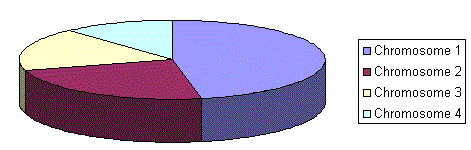
\includegraphics[width=4in]{intro/rwsgraph.png}
\caption{\label{fig:rwsgraph}Ruleta FPS}
\end{figure}

La sel·lecció \emph{basada en ranking}, és un altre mètode que intenta
solucionar els problemes de FPS \cite{B87a}.  Aquest mètode manté la pressió
selectiva ordenant la població en funció del seu fitness, i assignant les
probabilitats de sel·lecció en funció de la ordenació en comptes de fer-ho en
funció del propi fitness. D'aquesta manera, s'estableix una relació de qui és
millor que qui, però no hi ha els problemes que teniem en FPS.  El problema que
té aquest mètode és que no fa cap distinció entre les relacions de fitness
excepte per la relació de ser millor que un altre.  Per exemple, tres elements
amb fitness 1,2,3 s'ordenaran igual, i amb les mateixes probablilitats de ser
seleccionats que elements amb fitness 1,100 i 1000 .  La manera que es té de
mitigar (que no solucionar) aquest problema és asignar proporcions escalades en
relació entre la posició en el ranking i la probabilitat de ser sel·leccionat,
pot ser una relació lineal, exponencial o bé logarítmica. 

En la figura \ref{fig:rank1} es mostra  un cas on hi ha un cromosoma que tindria
el 90\% de probablilitats de ser escollit. El que es fa és ordenar de pitjor a
millor, i al pitjor donarli un ``calaix'', al següent dos, al següent tres, i
finalment, al millor quatre. 

\begin{figure} \centering 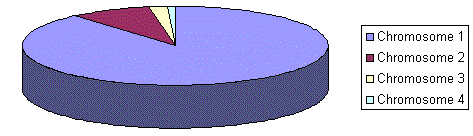
\includegraphics[width=4in]{intro/rank1.png}
\caption{\label{fig:rank1}seleccio ranking}
\end{figure}

En casos reals, s'utilitzen sistemes una mica més sofisticats, com per exemple
la \emph{sel·lecció per torneig}.  En una sel·lecció per torneig s'ha de definir
un paràmetre $N$ que descriu el tamany del torneig.

En la sel·lecció per torneig, per decidir quin individu passarà a la següent
generació, es realitzen ``enfrontaments'' de $N$ individuus, comparant el seu
fitness.  El que guanya de tots ells serà qui passarà a la fase de creuament.

Una de les avantatges que té aquest mètode és que no fa falta tenir
comptabilitzats tots els fitness de la població sencera, ja que només s'han
d'evaluar per grups de $N$.  Això el fa molt còmode d'usar en sistemes
paral·lelitzats, o bé en problemes on es molt costós fer una ordenació dels
fitness a nivell global, com per exemple, quan avaluem tirades en un joc
estratègic.

Hi ha variants de tornejos on, es defineix un altre paràmetre, que és la
probabilitat que el que té millor fitness surti realment guanyador.  En els
tornejos normals (deterministes), aquest parametre $p=1$, però si el disminuim
tal que $p<1$, hi haura un numero de casos $1-p$ on no guanyarà el millor.
Aquesta tècnica redueix la presió evolutiva permetent que individuus pitjors,
passin el seu codi genètic a següents generacions, augmentant la diversitat.

L'algorisme esquematitzat (tant per p=1 com per p<1) és el següent:

\begin{itemize}
	\item S'escullen $N$ individuus de la població aleatòriament.
	\item S'agafa el millor individu amb probabilitat $p$.
	\item S'agafa el segon millor individu amb probabilitat $p \times (1-p)$
	\item S'agafa el tercer millor individu amb probabilitat $p \times (1-p)^2$
	\item \ldots
\end{itemize}


En aquest projecte s'ha utilitzat una selecció \emph{stochastic
universal samplig} \cite{B87a} amb \emph{rank selection} \cite{B87b} i una
tècnica d'especiació coneguda com \emph{sharing} \cite{33}.

\subsubsection{Creuament}

Un cop s'han seleccionat els individus de la nova població, aquests podran tenir
descendència. Per a cadascun d'ells es genera un nombre aleatori entre 0 i 1, i
si no supera una determinada probabilitat de creuament, normalment bastant alta,
és copiat directament a la següent fase que és la mutació.

Els individus escollits per creuar-se són agrupats en parelles aleatòries, i
s'aplica un creuament clàssic discret unipunt.  Es genera un punt de tall del
cromosoma de forma aleatòria, i es construeixen dos descendents. El primer
descendent contindrà la primera part del material genètic del primer progenitor
fins el punt de tall, i la segona part del segon progenitor, que va des del punt
de tall fins el final del cromosoma. El segon descendent serà a l'inrevés, la
primera part serà directament la primera part del segon progenitor, i la segona
part la segona del primer progenitor.

En els dos problemes de GA hem utilitzat el creuament unipunt, però també hi
ha variants d'aquest creuament utilitzant dos o més punts.  Com es veurà en les
seccions de cadascun dels problemes, s'han fet proves amb aquests creuaments,
però no ens han donat resultats millors, i hem seguit amb els creuaments
unipunt.

Aquests creuaments, es poden aplicar amb seguretat quan considerem que la
relació d'un gen $i$ amb el gen $i+1$ no és forta.  Si trencant un cromosoma per
la posició $i$, destruim algun \emph{building block}, probablement, es perdrà un
factor que feia que l'individu fós bo, i al creuar-lo, no obtindrem gaire bons
resultats.

\subsubsection{Mutació}

Finalment, abans de tancar el cicle, es realitza la mutació. Aquesta activitat
aplica mutacions de forma aleatòria, però amb una baixa probabilitat, als gens
dels individus de la nova generació que està a punt de crear-se. En el cas de
disposar d'elitisme, aquests individus no són exposats a les mutacions.

L'operador de mutació emprat és clàssic uniforme. Això implica que els gens
seleccionats per a ser mutats, se'ls canvia el seu valor de forma aleatòria
però, el nou valor pertany al domini de la variable de decisió que codifica
aquell gen.

\subsubsection{Reemplaçament}

El model de reemplaçament seleccionat és el conegut com elitisme, que com ja
s'ha explicat abans, crear tota una nova població d'individus de generació en
generació. Malgrat això els $k$ millors individus van guardant-se per tal
d'assegurar que no es perden al llarg del procés evolutiu.  En tots els
projectes que es presenten en aquest treball, s'ha mantingut la mida de la
població, però també es possible fer que les mides de la població variin al
llarg de les generacions.

%\subsection{Teoremes} En general no n'hi ha cap teoria universalment acceptada
%del perquè funcionen bé els GA, ni del perquè de la seua robustesa. Però n'hi
%han dues hipòtesis que són interessants conèixer per que ens poden ajudar a
%implementar bones aplicacions dels GA, i cada cop més estan adoptant-se pels
%teòrics com els vertader mecanismes que fan evolucionar els GA. El primer
%d'ells és el teorema de la disposició, i el segon la hipòtesi dels blocs de
%construcció, o \emph{building blocks}.

%\subsubsection{Teorema de la disposició} Més conegut per \emph{schema theorem},
%va ser proposat per Holland \cite{H75}. Un \emph{schemata} és un patró de
%valors dels gens en binari. On aquest patró està format \{1, 0, \( \star  \)\}
%sent \( \star  \) el caràcter comodí. De tal forma que cromosomes com
%{}``0000'', {}``0010'', {}``0001'' i {}``0011'' corresponen al mateix patró
%{}``00\( \star \star  \)''.

%Aquest teorema diu que els individus bons, ho són per que tenen un bon patró.
%Llavors hem de donar-los a aquests individus més possibilitats de reproducció
%en funció del seu \emph{fitness}.  Per tant al passar aquests patrons a la
%descendència i al aplicar-los aquest mateixa filosofia, anem augmentant les
%possibilitats de generar millors patrons a mesura que passa el temps.

%Segons Holland si distribuïm aquestes probabilitats en funció de la proporció
%del \emph{fitness} d'un individu a seleccionar front al de la resta, un bon
%patrons estarà tenint un nombre de possibilitats que va creixent
%exponencialment. També va dir que el nombre de patrons que estant sent
%processats en una generació, és n\( ^{3} \), on n és el tamany de la població.
%Això és conegut com paral·lelisme implícit.

%\subsubsection{Hipòtesi sobre els blocs de construcció \label{subsec:bb}}
%Goldberg, en canvi, formula la \emph{Building Block Hypotesis} \cite{G89}.  Que
%diu que la potència dels GA's recau sobre l'habilitat de crear bons blocs de
%construcció. Aquests són curts patrons amb una longitud fixa, que funcionen
%molt bé per separat; independentment de la resta del cromosoma. I que si se li
%és incorporat un bon bloc de construcció a un cert individu, el seu
%\emph{fitness} augmenta. 

%Per afavorir la aparició de blocs de construcció, la codificació del cromosoma
%hauria de tenir propers els gens relacionats, i al mateix temps, que la
%interacció entre els gens siga mínima.

%La no interacció entre gens vol dir que l'aportació d'un gen al còmput del
%\emph{fitness} no es vegi afectat per els valors que poden prendre altres gens.
%Més tard Goldberg va publicar els estudis teòrics sobre gens que sí que
%interaccionen entre ells i com aprendre aquestes interaccions
%\cite{Goldberg:2002}, això és conegut com \emph{linkage learning}, i amb
%l'algorisme BOA que en la secció \ref{EDA} s'explicarà, es poden arribar a
%salvara aquest tipus d'inconveniències. Cal dir que en aquest projecte el
%còmput del \emph{fitness} si que s'espera que es veja afectat per la
%interrelació entre gens.

\section{Programació d'expressions genètiques} % (fold)
\label{sec:Programacio d'expressions genetiques}

La Programació d'expressions genètiques(GEP), podríem dir que és una evolució de
la Programació genètica (GP) en tant que intenta solucionar el mateix tipus de
problema.  A diferència dels GA clàssics, que tracten de solucionar (al menys de
forma natural) problemes d'optimització, tant GP com GEP podríen ser
classificats dins dels algorismes d'aprenentatge.  Per posar un exemple, en la
majoria de GA, el que es busca optimitzar és una entrada per a un procés
\ref{fig:ch1-4}.  En canvi, en GEP i GP el que es busca és un procés que
optimitzi una entrada donada \ref{fig:ch1-5}.

\begin{figure} \centering 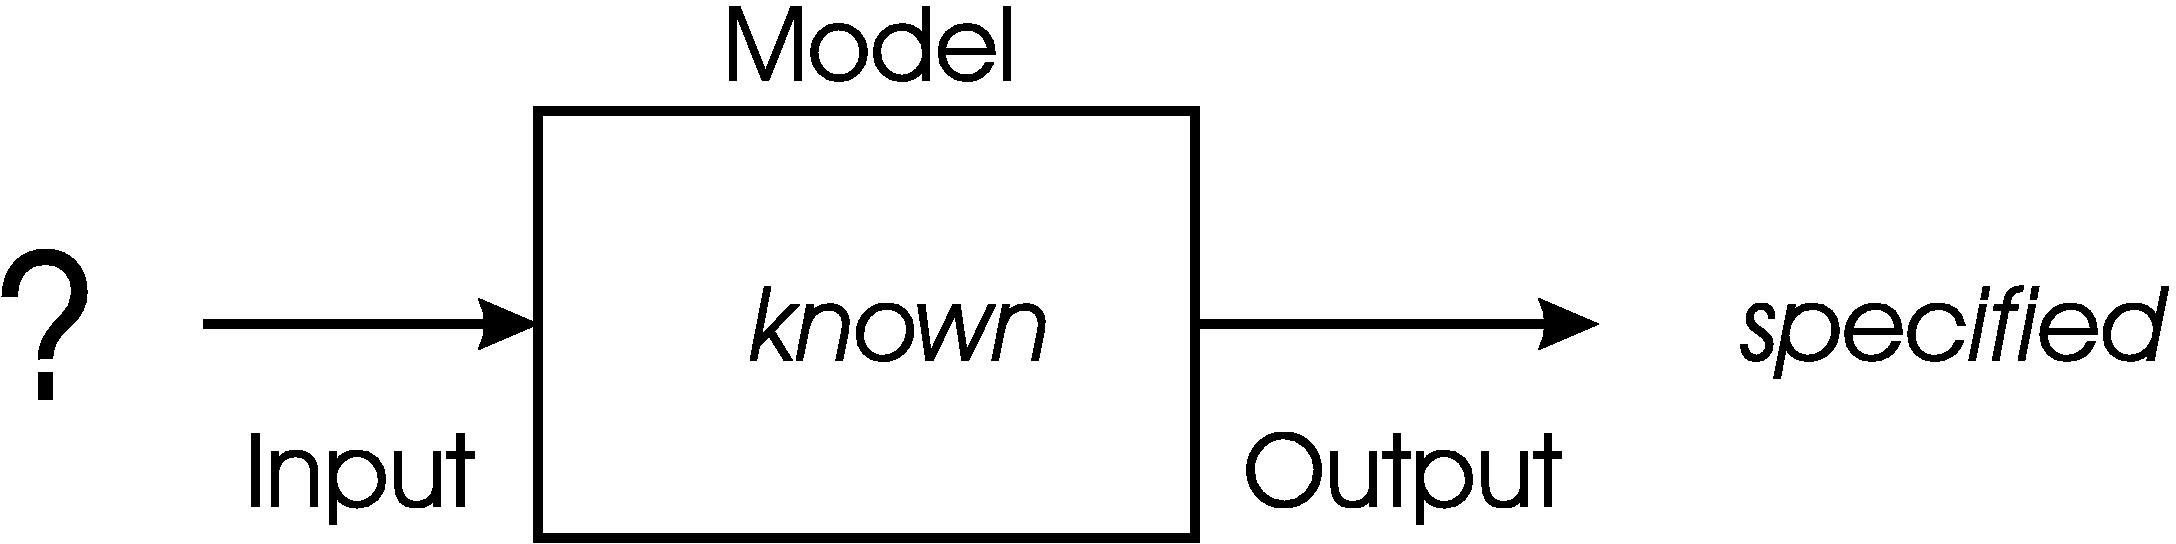
\includegraphics[width=4in]{intro/1-4.jpg}
\caption{\label{fig:ch1-4}Optimització d'entrada}
\end{figure}
\begin{figure} \centering 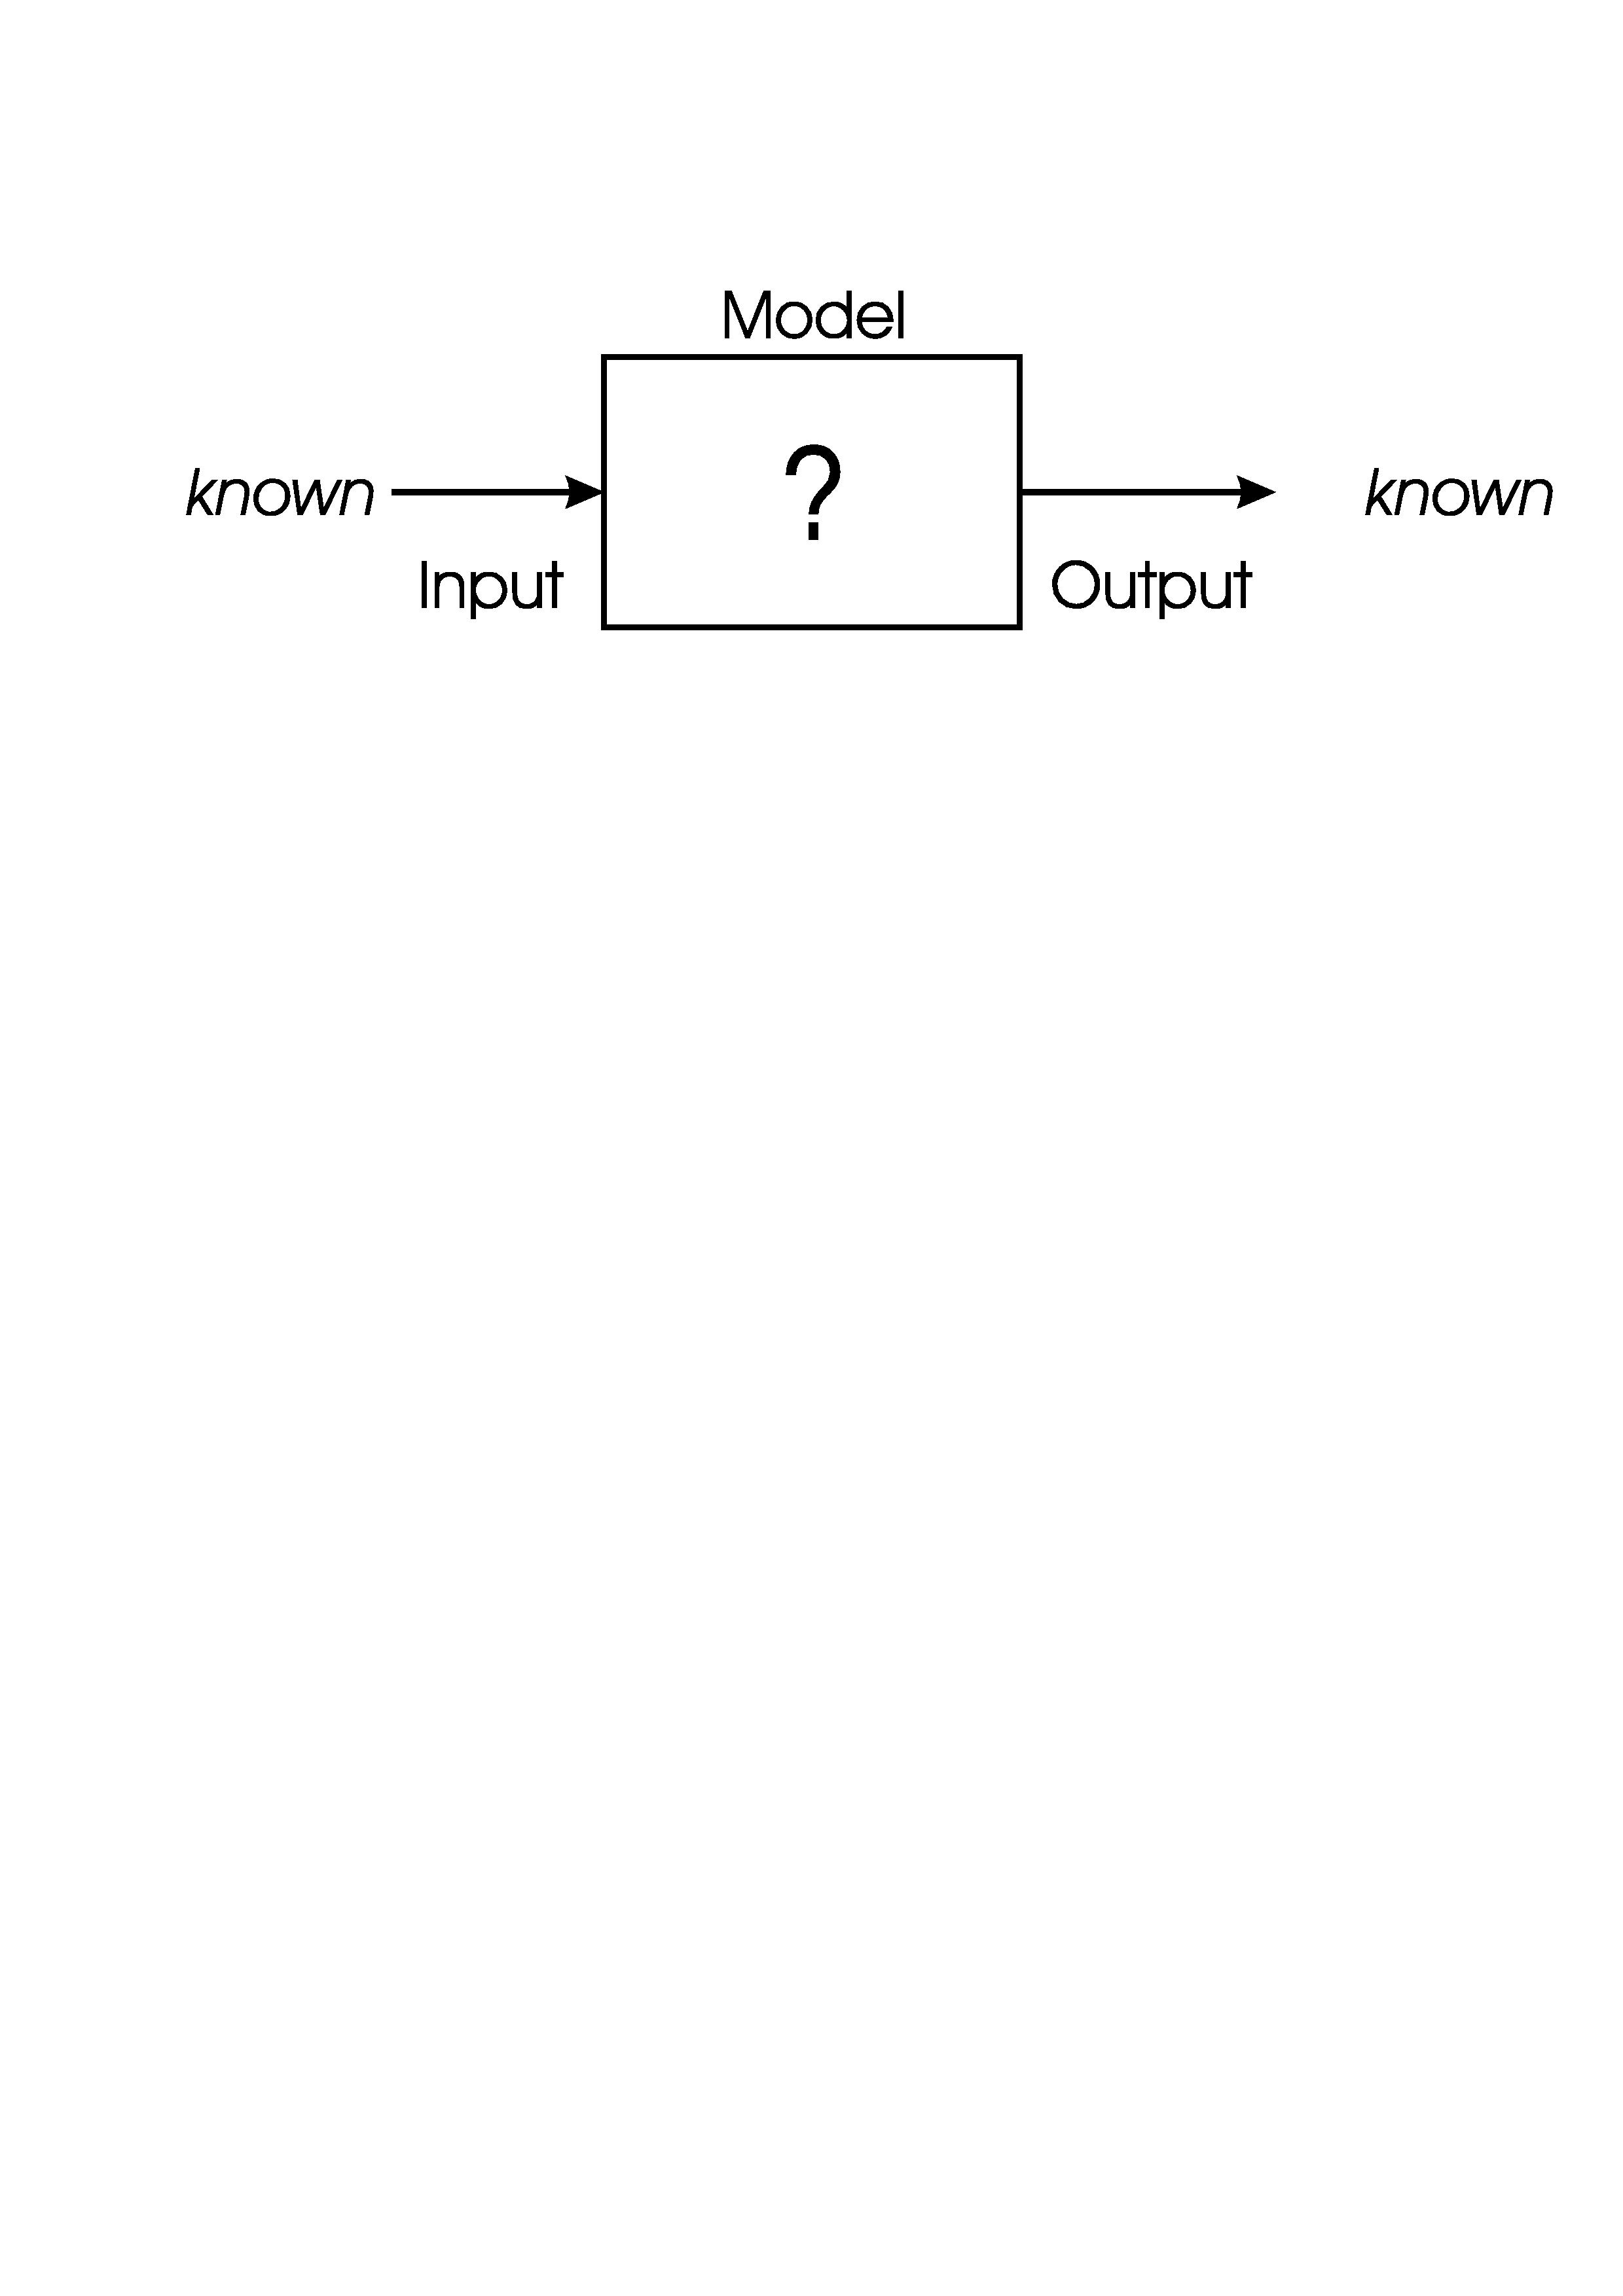
\includegraphics[width=4in]{intro/1-5.jpg}
\caption{\label{fig:ch1-5}Optimització procés}
\end{figure}

Els procéssos que s'intenten optimitzar, contenen, és clar, molta més informació
que en un dels algorismes genètics dels que s'han vist fins ara.  Això és
evident, ja que aquí, els individuus són parts funcionals d'un sistema i no
solsament dades que un sistema agafarà i evaluarà.  Tot seguit es mostren tres
exemples de possibles problemes que es poden voler optimitzar:

\begin{itemize}
	\item Fórmules lògiques (per exemple $ (x\land true) \rightarrow ((x \lor y)
	\lor (z \leftrightarrow ( x \land y)))$ )
	\item Fórmules aritmètiques (per exemple $2\times\pi+((x+3)-\frac{y}{5+1})$ )
	\item Programes 
		\begin{verbatim}
				i = 1;
				while (i<20){
					i = i + 1;
					}
		\end{verbatim}
\end{itemize}

\begin{figure} \centering 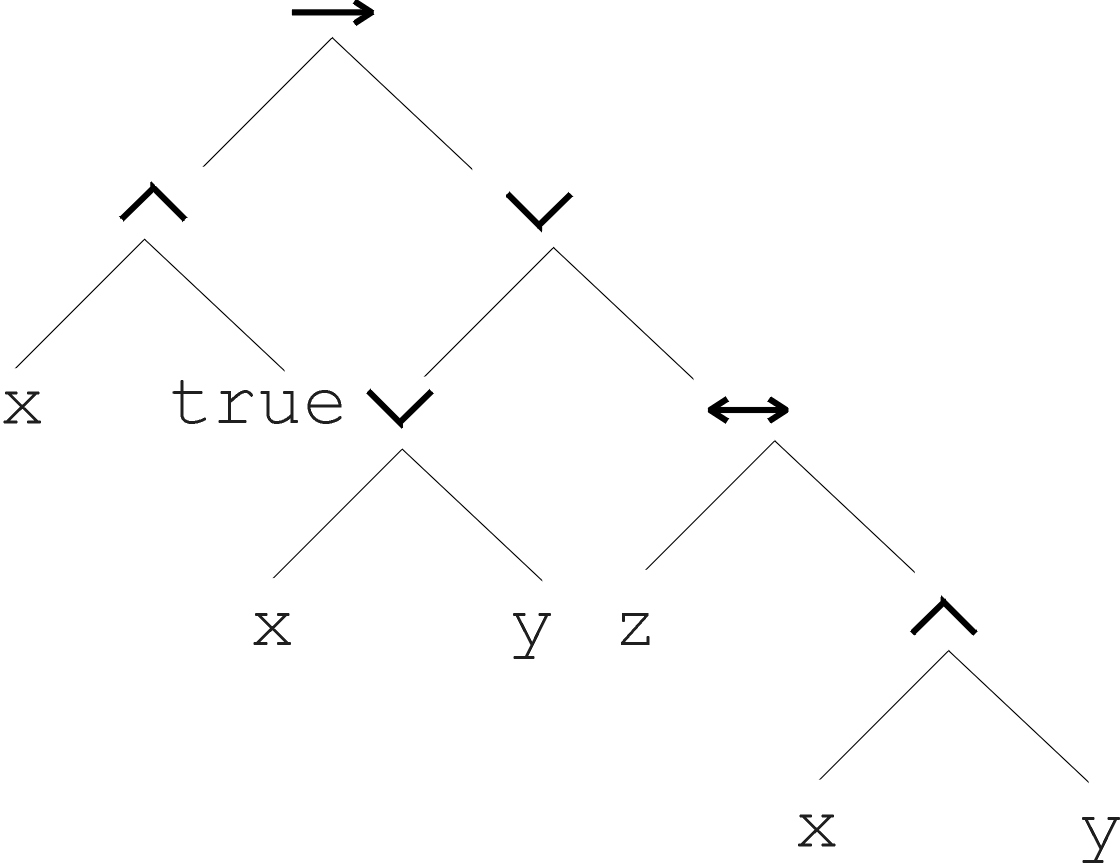
\includegraphics[width=4in]{intro/6-2-2.jpg}
\caption{\label{fig:6-2-2}Fórmula logica}
\end{figure}

\begin{figure} \centering 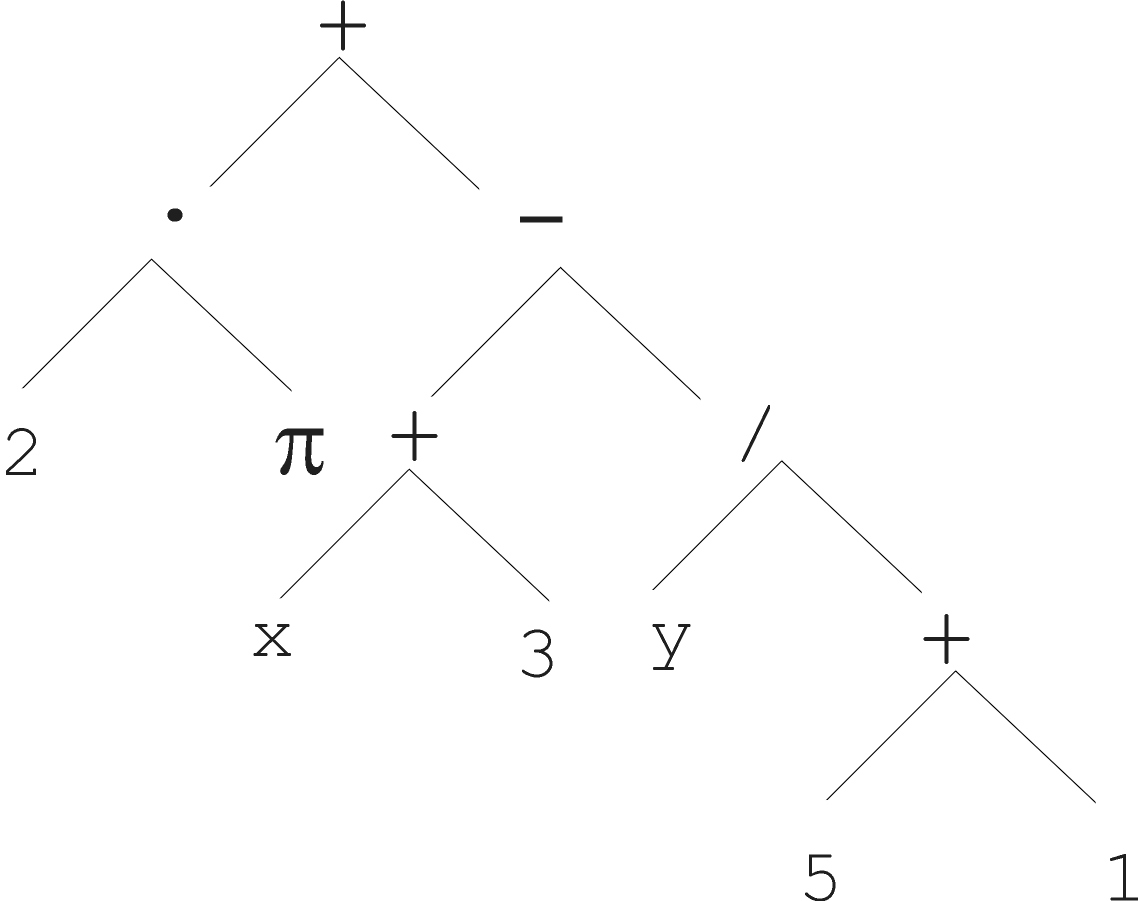
\includegraphics[width=4in]{intro/6-2-1.jpg}
\caption{\label{fig:6-2-1}Fórmula aritmètica}
\end{figure}

\begin{figure} \centering 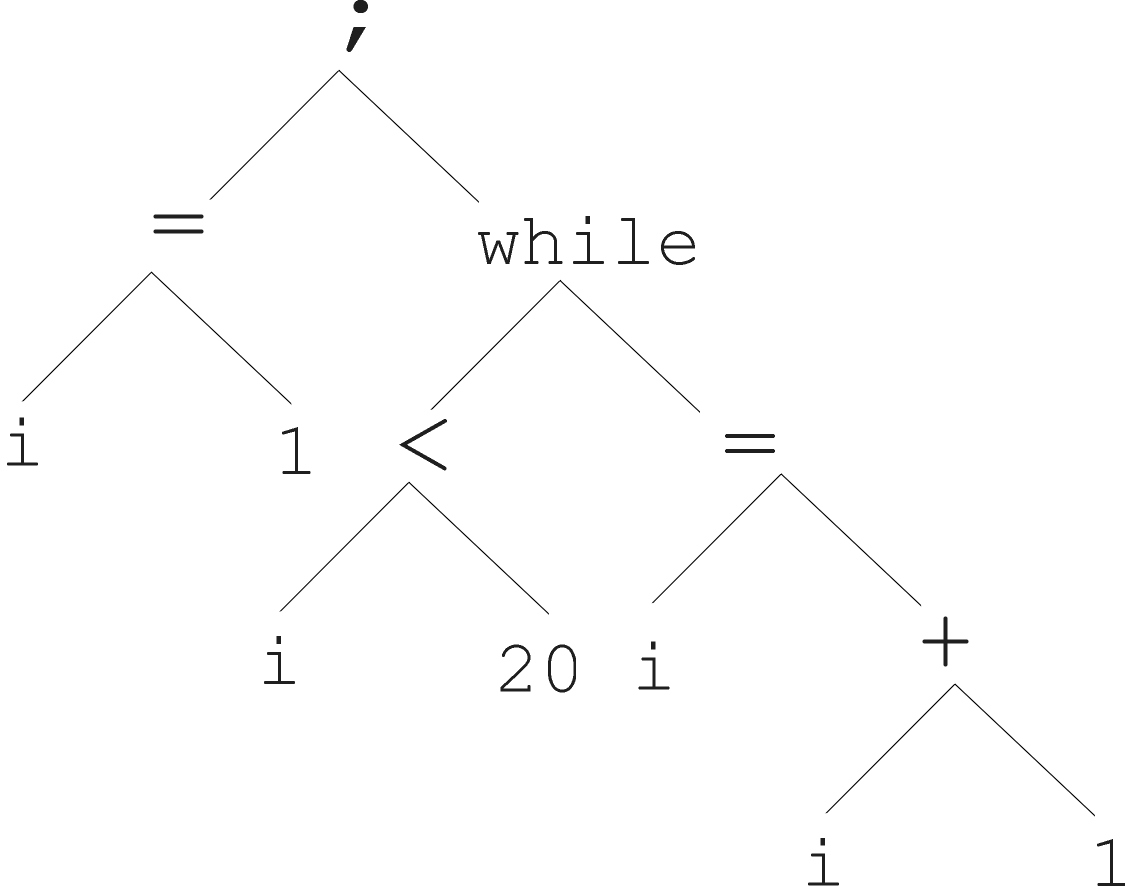
\includegraphics[width=4in]{intro/6-3.jpg}
\caption{\label{fig:6-3}programa}
\end{figure}
En aquest tipus d'algorismes, els individuus no poden ser codificats com a un
sol vector de bits o reals, i aquests ser tractats independentment uns dels
altres, sinó que el que han de codificar els individuus són arbres.  Per tant,
la seva codificació és més complexa, havent-hi una clara separació entre genotip
i fenotip.

Estrictament parlant, però, no hi ha cap altra diferència entre els GA clàssics
i GP o GEP.  Simplement, aquí interpretem els cromosomes com a arbres.

A continuació es farà una breu introducció a GP, per saber els antecesors de
GEP, i seguirà una explicació una mica més detallada de GEP, que és la tècnica
que s'ha utilitzat en \texttt{GEP}.

\subsection{Antecessors: Programació Genètica} % (fold)
\label{sub:Ant. Programacio Genetica}
La programació genètica és una de les diferents disciplines dins dels Algorismes
evolutius, inventat per Cramer en el 1085 (\cite{XX}) i després millorat per
John Koza en 1992 (\cite{XXX}) basat en la solució de problemes amb genotips de
llargada fixe, però interpretats de forma no lineal (arbres) de tamany i formes.

Els individuus en GP, normalment tenen un alfabet més ric que els AE classics,
però aquesta riquesta que ofereix tractar els cromosomes amb una interpretació
no lineal, fa que aquests individuus no siguin autònoms, i no poden funcionar
com a genotip i fenotip alhora, ja que han de passar per una fase de
``traducció''.

\subsubsection{Funcionament bàsic} % (fold)
\label{ssub:Funcionament basic}
% subsubsection Funcionament bàsic (end)

\subsubsection{operadors} % (fold)
\label{ssub:operadors}

Els algorismes de Programacio genètica tenen els mateixos operadors que els
altres AE, però amb la diferència notable que s'ha de tenir en compte que al fer
una modificació sobre el genotip, el fenotip pot veure's modificat de manera
``no prevista'' si no anem molt en compte.  Per exemple, al fer un creuament
entre dos individuus, el cromosoma resultant, pot no mantenir cap (o gairebé
cap) característica dels seus pares, donada la no-linealitat dels fenotips
respecte els genotips.  Això dona lloc a que molts dels individuus generats a
partir de individuus vàlids, són invàlids en el sentit que poden no complir les
condicions bàsiques per a ser traduits a fenotips i posteriorment evaluats.

Una manera de asegurar que les propietats dels progenitors es mantenen a la
descendència i que continuen éssent individuus vàlids, és aplicar els operadors
a nivell de fenotip, i assegurant-se que els fills continuen tenint una mínima
entitat que els fa evaluables en el context del problema.  Això dificulta molt,
però, la programació dels operadors.

Per exemple, en el cas d'interpretar els genotips com a arbres amb formules
matemàtiques, al fer creuaments podem fer-los per subarbres, agafant l'arrel i
el fill esquerra del arbre d'un dels dos progenitors, i el fill dret de l'altre. 
% subsubsection operadors (end)
% subsection Ant. Programació Genètica (end)

\subsection{Principis Bàsics} % (fold)
\label{sub:Principis Basics}

En GEP, els principals elements son els cromosomes i els arbres d'expressions,
on els segons són la expresió del la informació ogenètica codificada en els
cromosomes.  Com en la natura, el procés de decodificació s'anomena
\emph{traducció}.

La correspondència d'un a l'altre ha de ser únivoca i hi ha unes regles que ens
permeten passar d'un a l'altra.  En la natura, aquesta traducció no és pas tant
fàcil, ja que no se sap gairebé res del genotip, si tenim només un fenotip, però
per a tenir una traducció fàcil dins de GEP, es disposa d'una notació anomenada
\emph{Karva Notation} que ens permet fer les traduccions en les dues direccions
fàcilment \ref{ssub:Notacio Karva}.

% explicar constants


%http://www.gene-expression-programming.com/Tutorial002.asp
\subsubsection{Notació Karva} % (fold)
\label{ssub:Notacio Karva}

La notació Karva, és una manera de representar qualsevol expressió matemàtica o
lògica de manera que es pugui traslladar a un arbre.\cite{ferreira:2001}

Les estructures lineals que conformen els individuus són els cromosomes, i cada
cromosoma té un o més gens, que aquí prenen un altre significat més ampli, no
referint-se als ``àtoms'' indivisibles (com en els AE que hem vist fins ara)
sinó que cada gen està associat a una K-expression. \cite{ferreira:2007}

Tot seguit es mostra un exemple d'un gen, i en \ref{fig:expression tree1} el seu Arbre d'expresió equivalent

\begin{center}
0123456    
+/*abcd
\end{center}

\begin{figure}[h]
\begin{center}
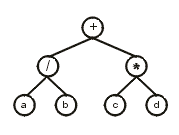
\includegraphics{intro/et1.png}
\end{center}
\caption{ET}
\label{fig:expression tree1}
\end{figure}

La traducció d'un a l'altre és directe.  El primer element en el gen (posició
0) correspon a la arrel del arbre.  Llavors, sota d'aquest node, s'enganxen
tants nodes fills com arguments tingui la funció representada pel node arrel
(dos en aquest cas). Els nodes fills es van omplint recursivament, consumint
simbols del cromosoma, fins que un nivell del arbre queda només omplert per
nodes terminals, que no son més que nodes on el símbol que contenen té aritat
zero.

Més formalment, tant el gen com l'arbre \ref{fig:expression tree1} poden ser
representats per la expresió matemàtica:

	$\frac{a}{b}+c \times d$

Per assegurar que els arbres que es crein siguin sintacticament vàlids,
es divideix un gen en dues parts, amb mides que segueixen unes normes
determinades.  Un gen es composa de la primera part (\emph{head}) que conté
funcions i terminals, i d'una segona part (\emph{tail}) que només conté
terminals (aritat zero). Si el tail és suficientment llarg com per omplir la
última capa del arbre que genera el propi gen, sempre hi haurà prous operands
per a donar a les funcions.

% subsubsection Notació Karva (end)

\subsubsection{Individus} % (fold)
\label{issub:individus}
% subsubsection individus (end)

COm s'ha explicat en \ref{ssub:Notacio Karva}, els individus son representats en
una tira de simbols (genotip), però al interpretar-los i evaluar-los, tenen una
representació en forma d'arbre d'expressió similar a un AST.

Un individu o cromosoma està format per un o més gens.  En la versió més
primaria, un cromosoma conté només un gen, però es poden combinar diversos gens,
creant cromosomes multigen, com s'explicarà més endavant.

En aquest tipus de notació, existeixen el que denominem ``zones
no-codificadores'', que són parts del gen, que per diversos motius formen part
del genotip, però no tenen representació, ni es mostren en el fenotip.  Un
exemple d'això és


\begin{verbatim}
	01234567890123456 	 
	Q/a*+b-cbabaccbac
\end{verbatim}

On la $Q$ representa l'arrel quadrada.  En aquest gen, té el i\emph{head} (que ocupa
de la posició 0 a la 7) de llargada, i el tail (de la 8 a la 16) de llargada 9.
El head té tant funcions com terminals, i el tail, només té terminals.

La codificació d'aquest gen es mostra en XXX (\ref{fda}) mostra com en aquest cas,
no han fet falta tots els elements del gen per a construir l'arbre.  Això és
perquè la fórmula que en assegura tenir prou tail, preveu el pitjor dels casos,
éssent tots els elements del head funcions amb la màxima aritat.  Com que en
aquest cas, tenim una arrel quadrada (i en l'arrel del arbre), deixem de
necessitar gairebé la meitat del gen per a fer la traducció.

Aquests trossos de cromosoma que no s'utilitzen, participen igualment en els
creuaments (es fan a nivell de vector de símbols), i fan que una mutació en una
zona del \emph{head} ``activi'' una zona prèviament inactiva.  Això dona tant
als creuaments com a les mutacions molta més versatilitat que en els algorismes
clàssics.

The beauty and elegance of the gene/ET system of Gene Expression Programming by itself is rather amazing, but most importantly it's that this is only the beginning and, indeed, this elegant genotype/phenotype system is at the heart of systems much more complex and also more efficient. In one such system the chromosomes contain more than one gene, and they are obviously called multigenic systems. In these systems, the chromosomes consist of multiple genes, and each gene codes for a sub-ET or sub-program. After translation, the sub-ETs are linked by special functions, the so called linking functions. These functions link the sub-ETs together one after the other in an orderly fashion. For example, the following chromosome composed of three genes (position 0 indicates the beginning of each gene):

012345678012345678012345678 	 

*aQ+abbaa/Q*/aababa*+Qaabba
	

(3)

codes for the three following sub-ETs:

Then the sub-ETs are afterwards linked by one of the available linking functions. For instance, if the linking function were addition, then the following program would be obtained (the linking function is shown in gray):

Note that the final program represented in the Figure above could be linearly encoded as a single K-expression:

01234567890123456 	 

++a*/aQQ*+/aaabba
	

(4)

However, the use of multigenic chromosomes is more appropriate to evolve solutions to complex problems, for they permit the modular construction of complex, hierarchical structures, where each gene codes for a smaller and simpler building block. These smaller building blocks are separated from one another and are therefore free to evolve independently, allowing for the creation of concrete new units that might prove handy in a new situation.

So, what is the use of Karva notation and why is it so important? The answer is that it allows adaptation or, in other words, learning: you replicate the linear strings of GEP, change a few bits, and you end up with new strings that encode slightly better programs. This is the basis for learning and evolution, and the plasticity of GEP genes with their noncoding regions allows the totally unconstrained exploration of the solution space, therefore increasing the odds of finding very good solutions to the problem at hand. No other programming system is as unconstrained as the genotype/phenotype GEP system in terms of the mechanisms used to create genetic variation (the Genetic Programming system is restricted to an inefficient tree-crossover and it's so complicated structurally that it never even developed beyond a single tree system [2]).

Furthermore, no other system has as much growth potential as GEP in the sense that the basic GEP system can give rise to other, more complex systems. We've already encountered here two GEP systems: the unigenic system and the multigenic system. But both these systems can be used as the starting point to create yet more complex systems: from simple GEP systems that elegantly handle random numerical constants to more sophisticated systems that can evolve highly complex structures such as neural networks, decision trees, automatically defined functions and polynomial networks. You can learn all about these and other GEP systems in Ferreira's book


\subsubsection{Esquema Bàsic} % (fold)
\label{ssub:Esquema Basic}
% subsubsection Esquema Bàsic (end)

\subsubsection{Funció d'avaluació} % (fold)
\label{ssub:funcio d'avaluacio}
% subsubsection funció d'evaluació (end)
% subsection Principis Bàsics (end)

\subsection{Operadors} % (fold)
\label{sub:Operadors}

\subsubsection{Inicialització} % (fold)
\label{ssub:Inicialitzacio}
% subsubsection Inicialització (end)

\subsubsection{Sel·lecció} % (fold)
\label{ssub:Seleccio}
% subsubsection Sel·lecció (end)

\subsubsection{Creuament} % (fold)
\label{ssub:Creuament}
% subsubsection Creuament (end)

\subsubsection{Mutació} % (fold)
\label{ssub:Mutacio}
% subsubsection Mutació (end)

\subsubsection{Reemplaçament} % (fold)
\label{ssub:Reemplacament}
% subsubsection Reemplaçament (end)

% subsection Operadors (end)




% section Programació d'expressions genètiques (end)

----END----

%\section{Algorismes genètics Lamarkians} Aquests algorismes en realitat són una
%combinació entre les teories evolutives Darwinistes i les Lamarkianes. Les
%teories evolutives Darwinistes han estat exposades en la secció anterior, i a
%grans trets aquestes es basen en la selecció natural. En canvi, les teories
%evolutives de Lamark que es recullen en el seu llibre \emph{Philosophie
%zoologique}, es basen en el fet de que les qualitats apreses al llarg de la vida
%d'un individu es transmeten per via genètica als seus descendents.

%Així doncs, en termes computacionals, els algorismes Lamarkians són uns
%algorismes genètics que fan evolucionar les poblacions mitjançant la selecció
%natural, però que just abans de generar nova descendència, cada individu pateix
%una serie de canvis individuals, que podrien ser vistes com una metàfora de la
%vida. És dir, que a cada individu se'l deixa viure i aprendre, i les bones
%qualitats apreses en aquest procés es transmetran als seus possibles
%descendents. D'aquesta manera un LGA funciona recoltzant-se en aquestes dues
%teories de l'evolució natural, i és per això que també son coneguts, com
%algorismes genètics híbrids, o fins i tot com \emph{memetic algorithms}.

%Aquest procés d'evolució individual s'intenta que sigui una optimització local.
%De tal manera que l'algorisme genètic realitza optimitzacions globals per
%l'espai de cerca, mentre que l'optimització individual es basa en una cerca molt
%local, i la combinació de les dues cerques fa que l'evolució de les solucions es
%realitzi de forma molt ràpida. En els annexos \ref{provesLGA} i \ref{provesEDA}
%es fa una comparativa entre un LGA i un GA, i LGA amb EDA, respectivament; En
%aquestes comparatives es pot veure un cert avantatge dels LGA respecte els
%altres algorismes (sempre amb el mateix nombre d'avaluacions per execució). En
%l'annex \ref{provesLGA} van ser utilitzades 20 funcions matemàtiques
%\emph{benchmark} \cite{YL97}, mentre que en l'annex \ref{provesEDA} es van
%utilitzar funcions del tipus \emph{deceptive trap} \cite{36} per fer les
%comparatives.

%L'optimització local que tots els individus pateixen, pot ser realitzada amb
%molts algorismes d'optimització. Els dos mètodes més habituals són el
%\emph{simulated annealing} \cite{AKM97} i estratègies evolutives
%\cite{Schwefel:1977}. Un estudi teòric molt complet sobre LGA usant estratègies
%evolutives  és el realitzat per Krasnogor \cite{K02}. Mentre que també es pot
%citar una aplicació usada en aquest projecte, que usa LGA amb \emph{simulated
%annealing} \cite{MGHHHBO98}.

%A banda dels passos evolutius locals, un LGA es comporta exactament igual que un
%GA dels explicats en la secció anterior. En la següent secció es detallaran amb
%més profunditat les estratègies evolutives, procés de cerca emprat pel LGA.

%\section{Estratègies evolutives} Les estratègies evolutives són un mètode
%d'optimització local que van ser proposades per primer cop per Schwefel
%\cite{Schwefel:1965}.  En els GA, el operadors bàsics són la selecció i el
%creuament, mentre que en les ES és la mutació la que juga aquest paper.  De fet,
%les propostes inicials de ES i la desenvolupada en aquest projecte, no té cap
%tipus de creuament. Més endavant ja es van proposar esquemes multimembrats amb
%diferents tipus de recombinacions \cite{37}.

%La notació utilitzada en  ES és $(\mu _,^+ \lambda)$.  On $\mu$ simbolitza el
%nombre d'individus de la població inicial en cada pas evolutiu. $\lambda$ el
%nombre final d'individus que es creen en cada pas evolutiu, la $,$ indica que
%sempre hi hauràreemplaçament, encara que els individus generats siguen pitjors
%que els pares, i $+$ indica que sols hi haurà reemplaçament si els individus
%generats són millors que els pares. L'estratègia evolutiva desenvolupada com a
%pas d'optimització local dintre del LGA és de l'estil $(1+1)$, és dir cada
%individu té un procés evolutiu independent de la resta, i sols serà dut a terme
%si el resultat supera l'inidividu inicial.

%A l'annex \ref{provesES} es poden consultar les proves realitzades a les ES
%desenvolupades sobre 20 problemes matemàtics típics en benchmarks d'aquest estil
%\cite{YL97}.

%\subsection{Representació dels individus\label{subsec:representacio}} Un
%individu està format per dos vectors, $\vec{a}=(\vec{x},\vec{\sigma})$. On
%$\vec{x} \in \Re^n$ és el vector que conté la informació del cromosoma és dir la
%informació que caracteritza cada fenotip; mentre que $\vec{\sigma}$ conté
%informació necessària per la ES per realitzar la mutació.

%El vector $\vec{\sigma} \in \Re^n$ són les desviacions típiques amb que són
%realitzades les mutacions Gaussianes (veure apartat \ref{subsec:ESmut}) sobre
%cada un dels gens de l'individu. Aquest vector s'inicialitza aleatòriament i va
%evolucionant junt amb el mateix cromosoma, de tal forma que el sistema va
%aprenent quina és la forma més òptima de realitzar les mutacions.

%En casos bastant particulars també s'inclou dintre del vector $\vec{a}$ un
%tercer vector que conté els angles de rotació amb que seran tractades cada una
%de les desviacions típiques per fer-les evolucionar. En aquest cas no s'ha
%inclòs ja que la complexitat de la cerca augmenta de forma exponencial amb la
%inclusió de nous valors a optimitzar dintre del problema, i cal fer notar que
%els passos evolutius que realitza un LGA són de l'ordre de 5, amb la qual cosa
%no donaria temps a optimitzar gaire cosa.

%\subsection{Esquema bàsic}

%L'esquema de funcionament d'una estratègia evolutiva $(1+1)$ es pot resumir en
%la figura \ref{fig:es}. A l'inici de l'estratègia, a l'individu se li fan una
%serie de mutacions Gaussianes que a l'apartat \ref{subsec:ESmut} seran
%explicades. A continuació s'avalua el nou individu generat. I sols si el nou
%individu és millor que l'inicial, el nou substitueix a l'inicial, si no ho és,
%torna a realitzar altra mutació sobre l'inicial, és dir, que sols hi ha
%reemplaçament si el nou individu supera a l'inicial o d'altra forma, es manté
%una filosofia elitista. Aquest bucle es realitza tants cops com passos evolutius
%hi hagen definits.

%\begin{figure} \centering 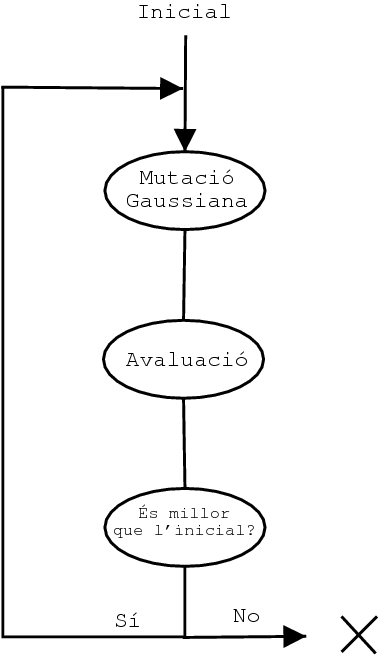
\includegraphics[height=4in]{es}
%\caption{\label{fig:es}Diagrama d'activitats d'una estratègia evolutiva}
%\end{figure}

%\subsection{Selecció i reemplaçament} La selecció en ES és determinista. Sempre
%es seleccionen els millors individus de la població, però per fer-ho hi ha dues
%formes diferents, l'elitista i la no elitista. En l'elitista, que és la versió
%utilitzada en aquest projecte, es seleccionen els millors individus del conjunt
%format pels individus inicials més els nous individus. En la no elitista sempre
%es seleccionen els individus del nou conjunt generat.  Seguint la notació de les
%ES, $(\mu _,^+ \lambda)$, en el model elitista s'escolliran els $\mu$ millors
%individus de la població total (inicials i nous), mentre que en el model no
%elitista sols s'escolliran el $\mu$ millors individus sobre els $\lambda$ nous
%individus creats, d'ací ve la restricció en que $\mu < \lambda$.

%Experimentalment s'ha reportat que el model elitista fa augmentar la velocitat
%de convergència i assegura que mai es perden individus bons \cite{OBS98}.

%\subsection{Mutació\label{subsec:ESmut}} La mutació és el pilar bàsic sobre el
%qual es recolzen les ES. En les ES la mutació utilitzada és Gaussiana, i
%mitjançant variables aleatòries que segueixen una distribució normal, es simula
%de certa manera un entorn natural en tant i en quant, les mutacions xicotetes es
%realitzen molt a sovint, però les grans mutacions són més poc freqüents.

%A més a més, aquest operador de mutació també fa evolucionar de manera conjunta
%a la solució, la desviació típica de cada gen, de manera que a cada pas evolutiu
%les mutacions realitzades sobre cada gen seran més òptimes, és dir, si es veu
%experimentalment que grans mutacions sobre un gen beneficien l'increment del
%\emph{fitness} total, llavors la desviació típica d'aquella mutació augmenta per
%a les següents mutacions, però si per el contrari, es veu que una variació sobre
%un gen concret fa disminuir el \emph{fitness}, la desviació típica baixa.

%Com es va comentar en l'apartat \ref{subsec:representacio}, un individu està
%format habitualment per dos vectors, $\vec{x}$ i $\vec{\sigma}$, i les equacions
%que regeixen les mutacions sobre aquests vectors són les següents: \[
%\vec{x}^\prime=\vec{x}+\vec{N}(\vec{0},\vec{\sigma}) \] \[
%\sigma_i^\prime=\sigma_i \cdot exp(\tau^\prime \cdot N(0,1) + \tau \cdot
%N_i(0,1)) \]

%Pel que fa a la mutació de $\vec{x}$, a cada gen de l'individu inicial se li
%suma un un nombre aleatori que segueix una distribució normal, amb mitjana 0 i
%desviació típica $\sigma$, això és el que es simbolitza amb $N(0,\sigma)$.

%D'altra banda, la mutació de les desviacions típiques es veu afectada per dos
%termes, el primer que és comú per a totes les mutacions que es realitzen sobre
%les desviacions típiques, i el segon que és personalitzat per a cada desviació
%típica. El primer terme és un nombre aleatori amb mitjana 0 i desviació típica 1
%amb una distribució normal, multiplicat pel paràmetre $\tau^\prime$. I el segon,
%terme és un nombre aleatori amb mitjana 0 i desviació típica 1 amb una
%distribució normal, multiplicat pel paràmetre $\tau$. $\tau^\prime$ i $\tau$ es
%recomana que siguen proporcionals als valors que es mostren a continuació
%\cite{Schwefel:1977}: \[ \tau \propto \frac{1}{\sqrt{2 \sqrt{n}}} \] \[
%\tau^\prime \propto \frac{1}{\sqrt{2n}} \]

%on, $n$ és la llargada del vector $\vec{x}$.

%A la secció \ref{subsec:representacio} també es va comentar que es poden afegir
%angles de rotació com un paràmetre extra del cromosoma. Això és degut a que
%alguns cops les mutacions ortogonals no són suficients i els individus s'han de
%desplaçar en diagonal per ser més eficients. Si els angles de rotació són
%afegits a la ES la mutació canvia una mica, per a més informació es pot
%consultar el llibre de Thomas Bäck \cite{37}.

%\subsection{Recombinació} Les ES també contemplen la possibilitat d'incorporar
%recombinació entre els individus, encara que aquest no és el cas, ja que en
%aquest projecte la ES ha estat desenvolupada com a procés evolutiu local dintre
%d'altre procés evolutiu global. No obstant això es faran un breu repàs sobre
%aquests tipus d'operadors.

%Al igual que en els GA, en ES hi ha diversos tipus de recombinació o creuament,
%la principal diferència és que un GA típicament es treballa sota atributs
%binaris, mentre que en ES es sol treballar amb atributs reals. És per aquest
%motiu que les recombinacions estan orientades cap a valors reals. Els operadors
%de recombinació més usats sota ES són: discret, discret panmític, intermig,
%intermig panmític, intermig generalitzat i intermig generalitzat panmític.

%\section{Especiació\label{sec:especiacio}} En els algorismes evolutius, molt
%sovint, la població tendeix a convergir cap als màxims de la solució, ja siga un
%màxim local o un màxim global. En els casos en que la població convergeix cap a
%màxims locals, no interessa que la població s'homogenitze, ja que això fa pedre
%el paral·lelisme implícit que aporten els algorismes evolutius. El cas ideal que
%es desitjaria, és aquell que un cop conegut un màxim local, l'algorisme continue
%buscant altres màxims.

%Per fer això, diverses tècniques poden ser usades. Una de les més comuns és
%l'especiació o \emph{niching}. I dintre d'aquesta família de tècniques, s'hi
%poden trobar tècniques com el \emph{sharing} \cite{33}, \emph{crowding}, etc.

%La tècnica que s'ha emprat en la implementació d'aquest projecte és el
%\emph{sharing}. Aquesta tècnica és podria explicar com una metàfora agafada de
%la natura, que evoca la compartició de recursos limitats de l'entorn o els
%efectes de la pressió demogràfica sobre els individus.  És dir que si una zona
%del territori està molt poblada, el \emph{fitness} de la població cau pel fet
%que han de compartir els recursos.

%En termes matemàtics podríem descriure el \emph{sharing} com: Si dos individus
%estan situats a una distància ($d_{ij}$) menor que el radi de \emph{sharing}
%($\sigma_{sh}$), el seu nou \emph{fitness} es modifica seguint la següent
%equació:

%\[ fitness_i=\sum\limits^{tamany}_{j=0,j \neq i}\phi(d_{i,j}) \]

%\[ \phi(d_{i,j})=\left\{ \begin{array}{ll}
%1-\left(\frac{d_{i,j}}{\sigma_{sh}}\right)^\alpha & d_{i,j}<\sigma_{sh}\\ 0 &
%altrament \end{array} \right.  \]

%on, $\alpha$ està fixat a 1, i $\sigma_{sh}$ s'ajusta normalment de forma
%empírica, en aquest cas val 0.3. Les distàncies en aquest cas no són símplement
%la resta entre els valors que prenen els gens, sinó que, com aquests valors són
%categòrics, s'ha implementat una funció distància que retorna les distàncies
%entre dos aminoàcids en funció de la hidrofobicitat i de la càrrega. Per veure a
%més informació sobre aquesta funció distància es pot consultar l'apartat
%\ref{subsec:distancies}.

%El \emph{Sharing} és un operador amb el qual es por regular de forma molt
%efectiva la pressió selectiva sobre la població. Sobre les solucions molt
%properes la pressió selectiva és molt alta, mentre que les solucions aïllades no
%ho és tant. Això pressiona a aquelles solucions semblants a que evolucionen cap
%a llocs diferents, forçant així una major exploració de l'espai de cerca.

%\section{Conclusions} En aquest capítol s'han descrit dos dels quatre algorismes
%utilitzats en aquest projecte. Un és el GA i l'altre el LGA. A més a més, també
%s'han explicat les ES que és un algorisme evolutiu dissenyat en aquest cas per
%fer evolucions locals sobre els individus de la població, utilitzades per un
%LGA. I finalment la tècnica d'especiació emprada per els quatre algorismes
%desenvolupats.

%A l'annex \ref{provesLGA} es poden veure les proves i comparatives entre els GA
%i LGA. D'altra banda en l'annex \ref{provesES} es mostren els resultats de les
%proves que s'han realitzat sobre les ES, l'objectiu d'aquests resultats no és
%altre que comprovar que les ES s'han programat correctament, és es dir que és
%una prova parcial del projecte.

%Finalment es comentarà que en les comparatives realitzades, el LGA generalment
%és millor que el GA, aquesta idea de barrejar optimitzacions locals amb
%optimitzacions globals ha tingut l'èxit presentat en la bibliografia
%relacionada. Ara l'objectiu és comparar-lo amb altres algorismes per la
%resolució de problemes que requereixen \emph{linkage learning} per resoldre el
%problema òptimament \cite{G02}.

%\bibliographystyle{unsrt} 
%\bibliography{bibliografia}
\end{document}
